\documentclass{article}
\usepackage{graphicx}
\usepackage{booktabs}
\usepackage{float}

\begin{document}

\section{Análisis de Rendimiento del Modelo}

El rendimiento del modelo YOLOv8 entrenado para la detección de billetes chilenos fue evaluado cuantitativamente utilizando las métricas estándar de detección de objetos. Los resultados, extraídos del proceso de entrenamiento y validación, demuestran una alta precisión y fiabilidad.

\subsection{Métricas de Detección}

La tabla \ref{tab:metricas_rendimiento} resume el rendimiento final del modelo en el conjunto de datos de validación después de 100 épocas de entrenamiento. El modelo alcanzó un \textbf{mAP@0.50 de 99.4\%}, lo que indica una capacidad de detección extremadamente alta y precisa.

\begin{table}[H]
    \centering
    \caption{Métricas finales de rendimiento del modelo de detección.}
    \label{tab:metricas_rendimiento}
    \begin{tabular}{lc}
        \toprule
        \textbf{Métrica} & \textbf{Valor} \\
        \midrule
        Precisión (Precision) & 99.2\% \\
        Recall (Sensibilidad) & 99.0\% \\
        mAP@0.50 & 99.4\% \\
        mAP@0.50-0.95 & 99.1\% \\
        \bottomrule
    \end{tabular}
\end{table}

\subsection{Análisis Gráfico del Entrenamiento}

La evolución del entrenamiento se puede observar en la figura \ref{fig:resultados_entrenamiento}. Los gráficos muestran una convergencia estable de las funciones de pérdida y un incremento consistente de las métricas de precisión y mAP, sin signos de sobreajuste.

\begin{figure}[H]
    \centering
    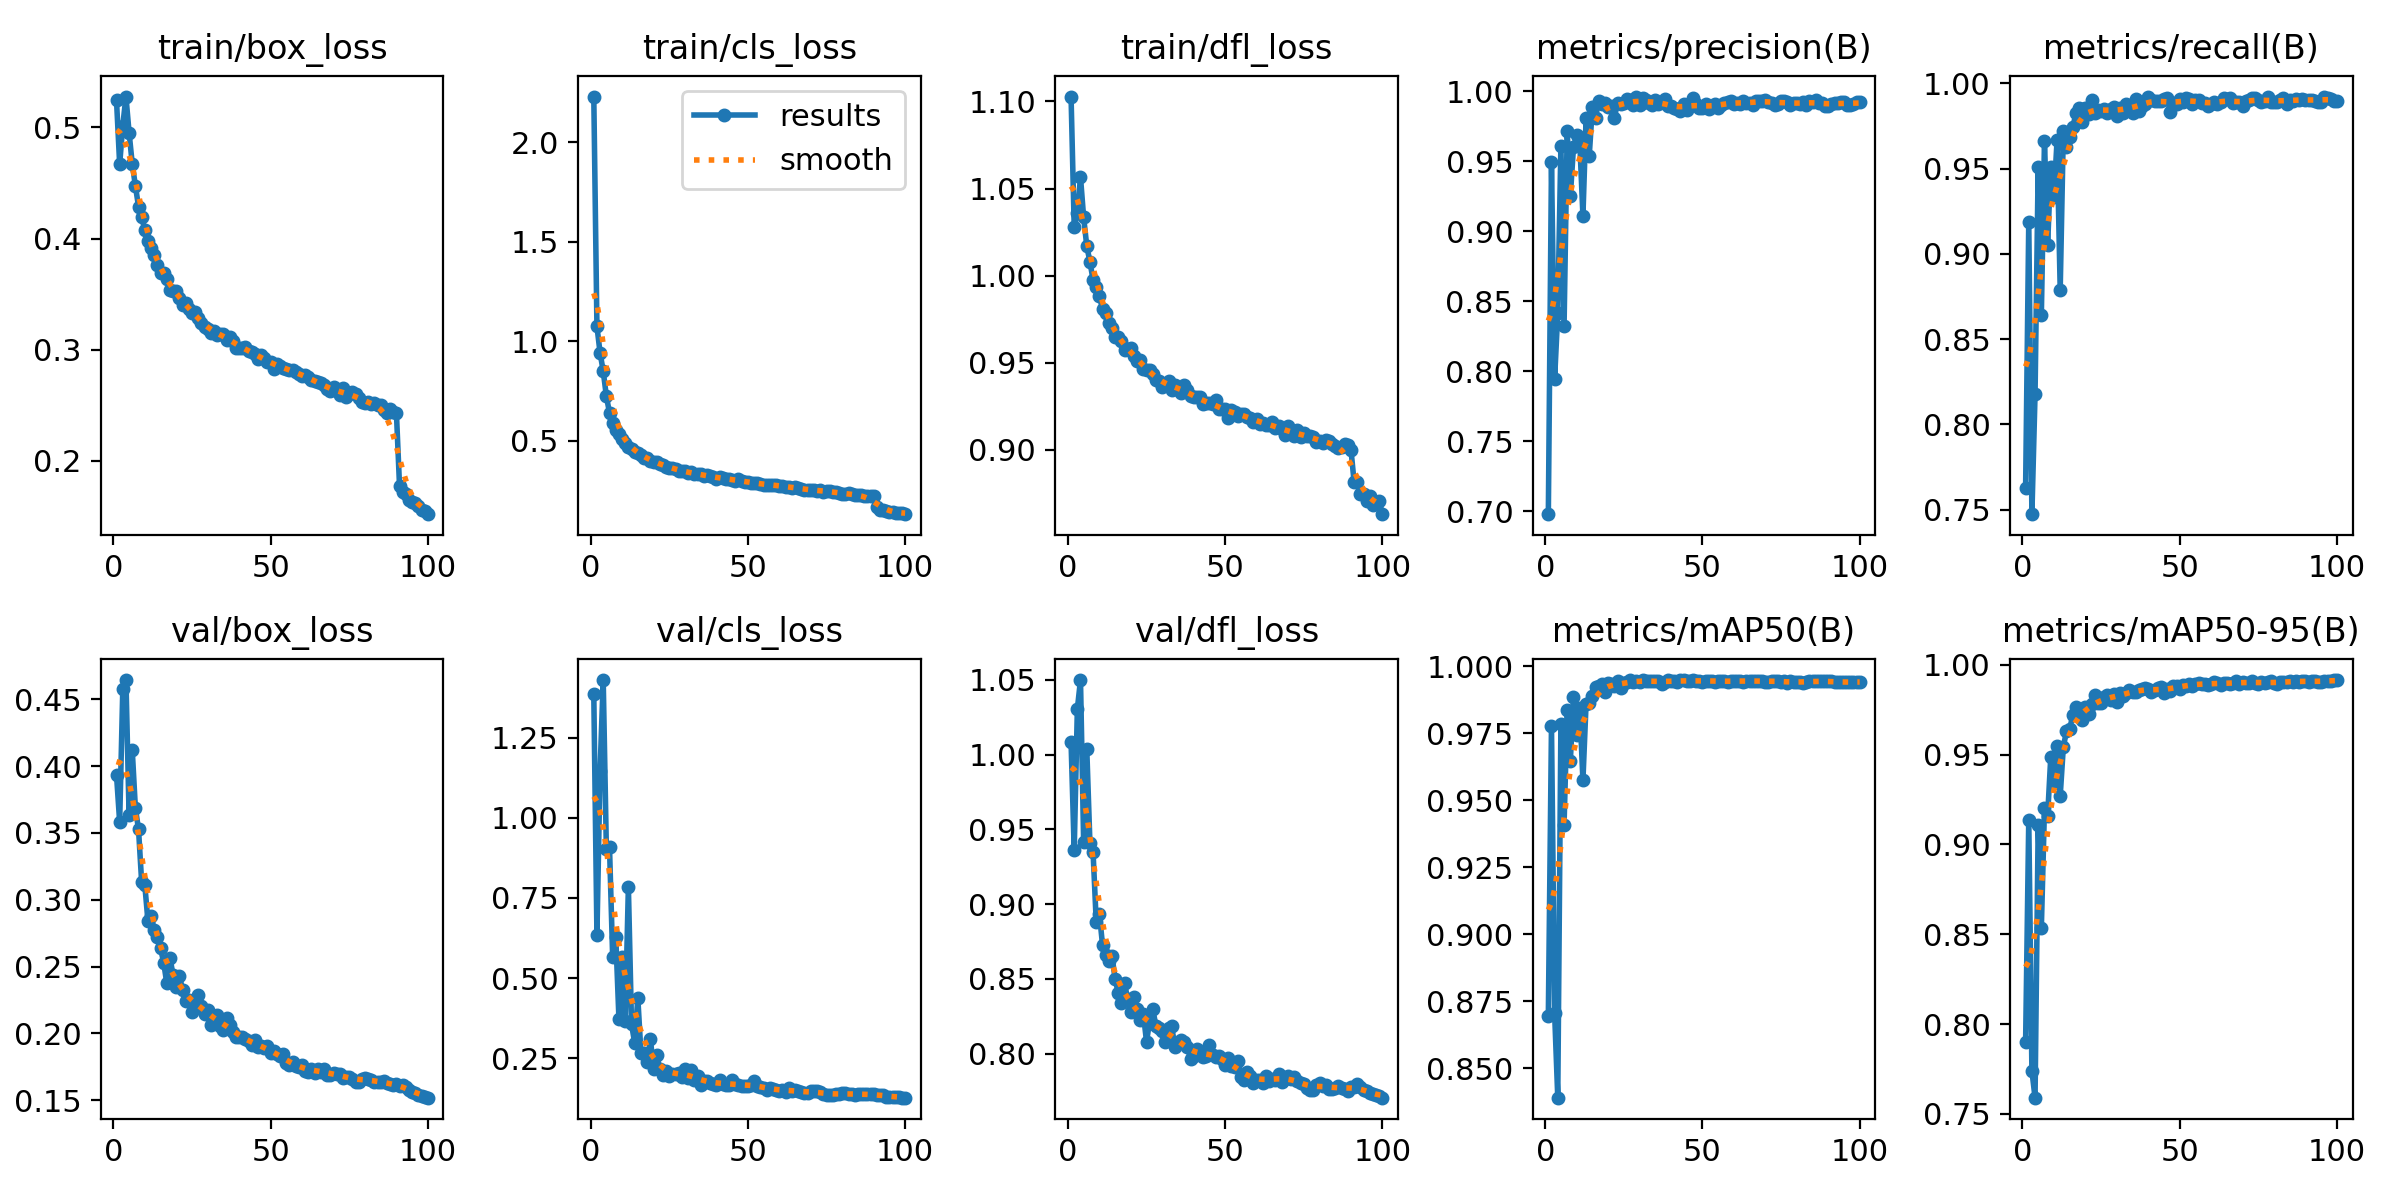
\includegraphics[width=\textwidth]{../DATASETS/runs/detect/train/results.png}
    \caption{Gráficos de resultados del entrenamiento, mostrando la evolución de las métricas y las pérdidas a lo largo de las 100 épocas.}
    \label{fig:resultados_entrenamiento}
\end{figure}

La curva de Precisión-Recall (figura \ref{fig:pr_curve}) y la matriz de confusión (figura \ref{fig:confusion_matrix}) refuerzan la conclusión de que el modelo es robusto, con un área bajo la curva cercana a 1 y una clara diagonal en la matriz, indicando pocas clasificaciones incorrectas.

\begin{figure}[H]
    \centering
    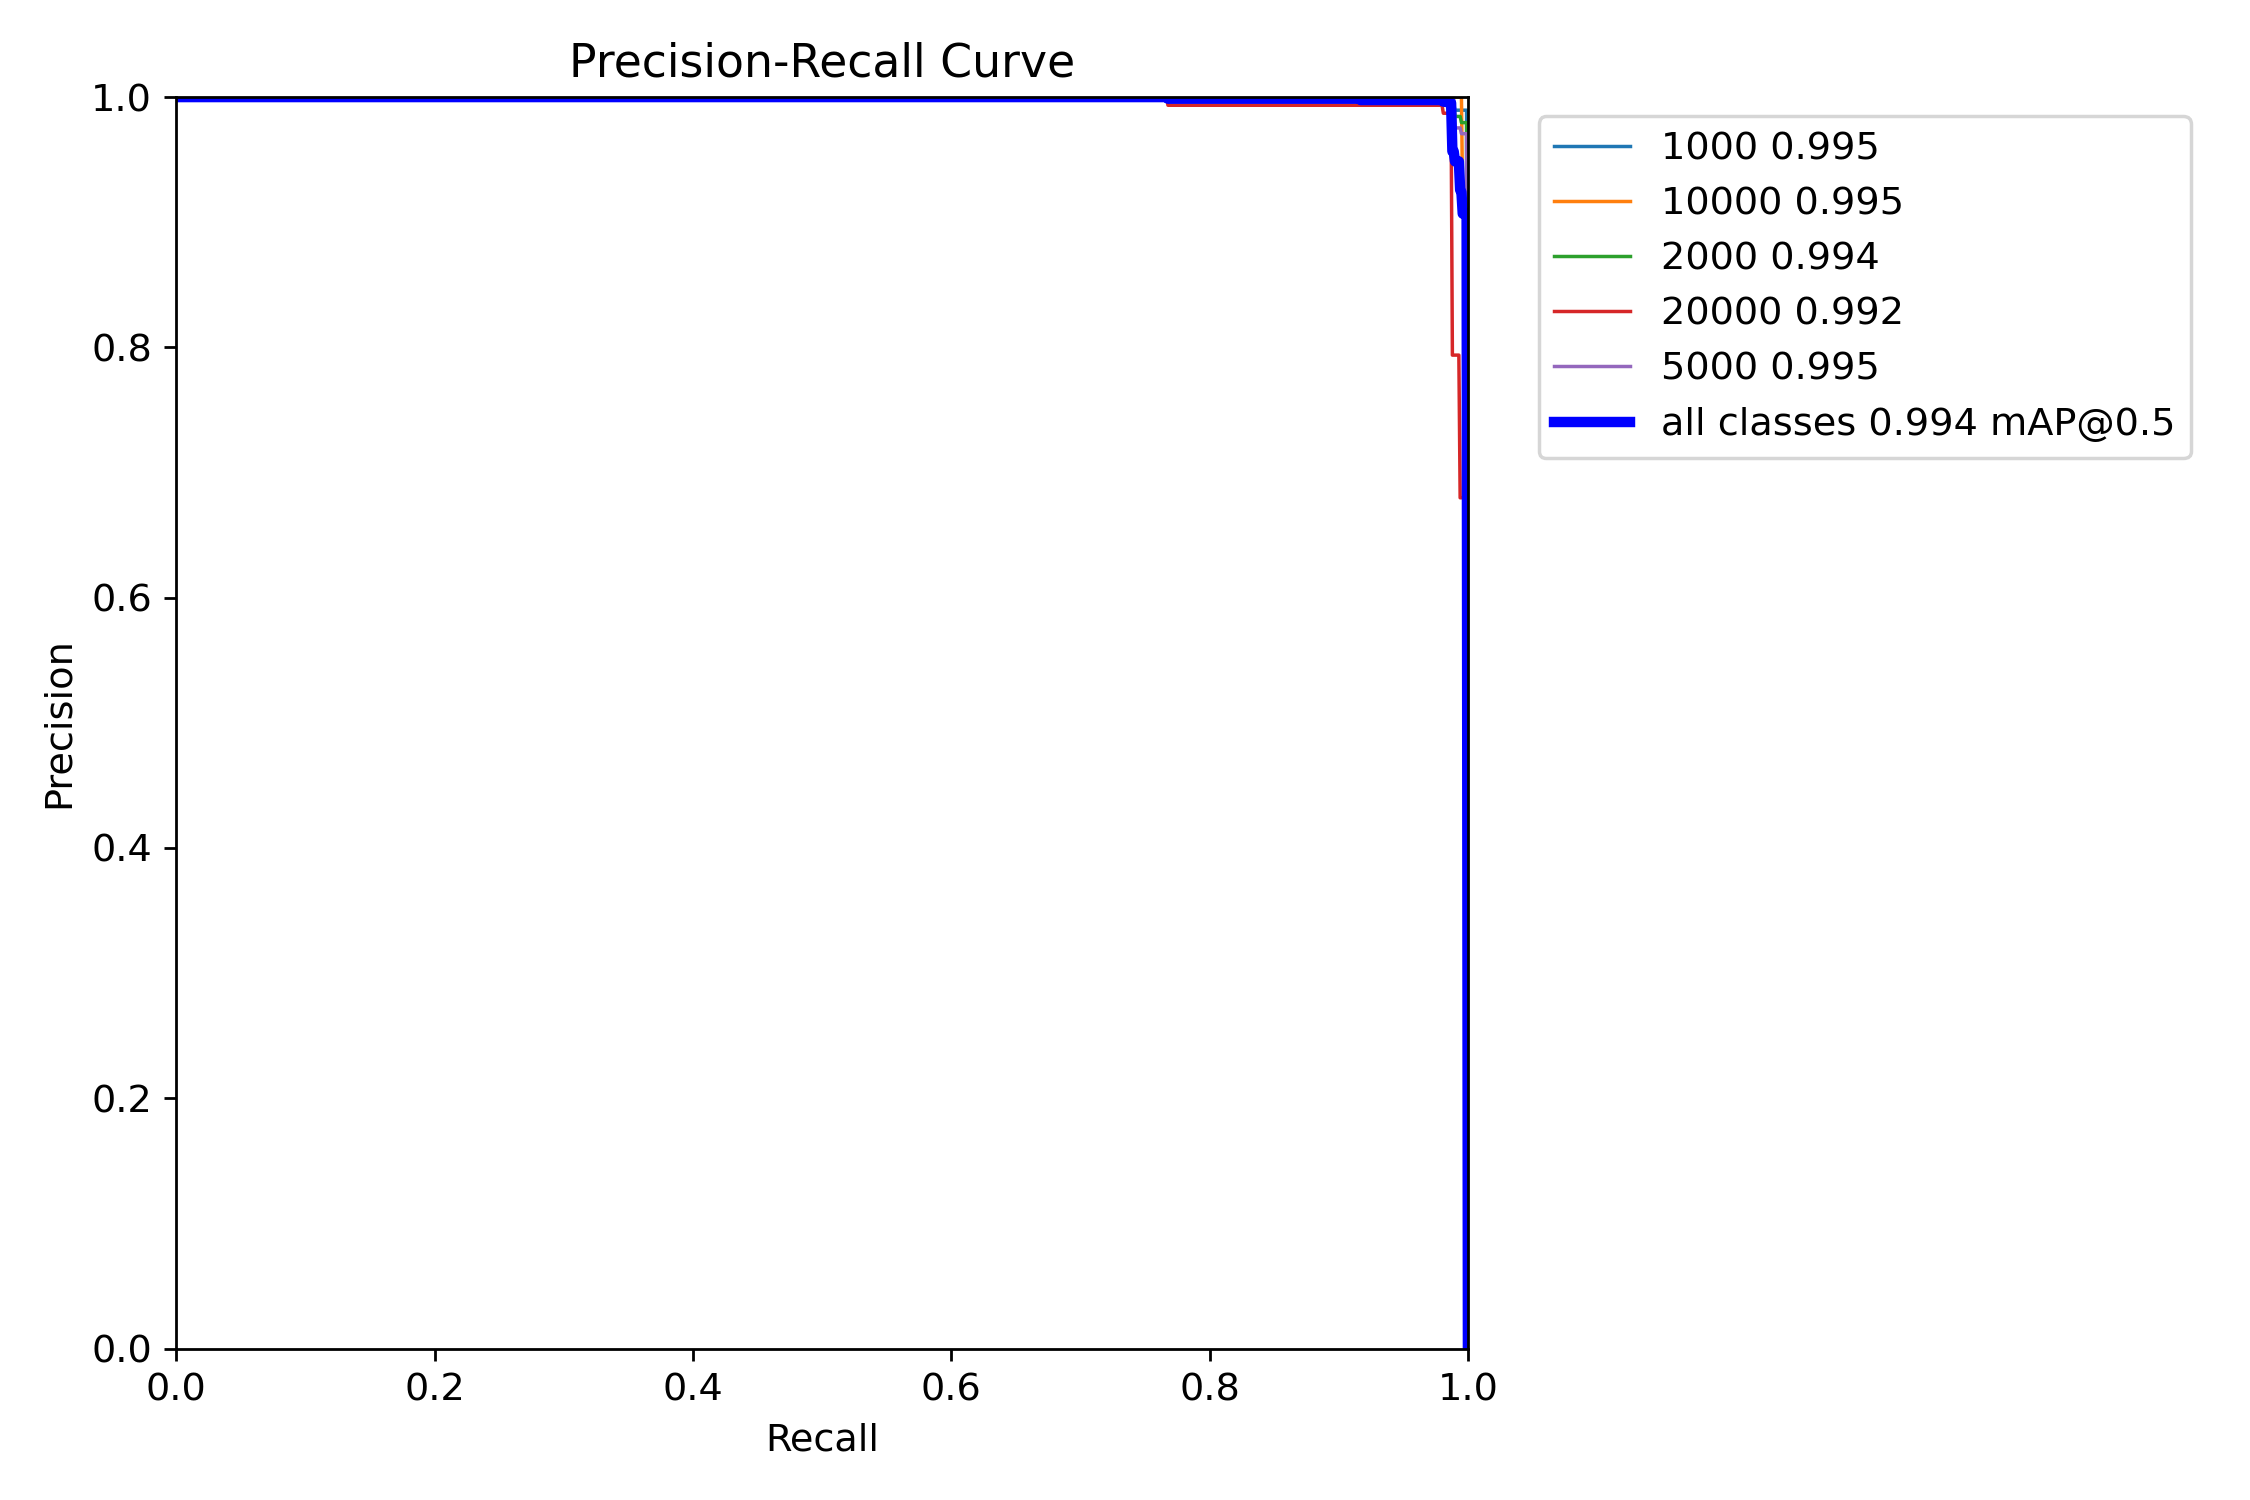
\includegraphics[width=0.8\textwidth]{../DATASETS/runs/detect/train/BoxPR_curve.png}
    \caption{Curva de Precisión-Recall (PR) para todas las clases.}
    \label{fig:pr_curve}
\end{figure}

\begin{figure}[H]
    \centering
    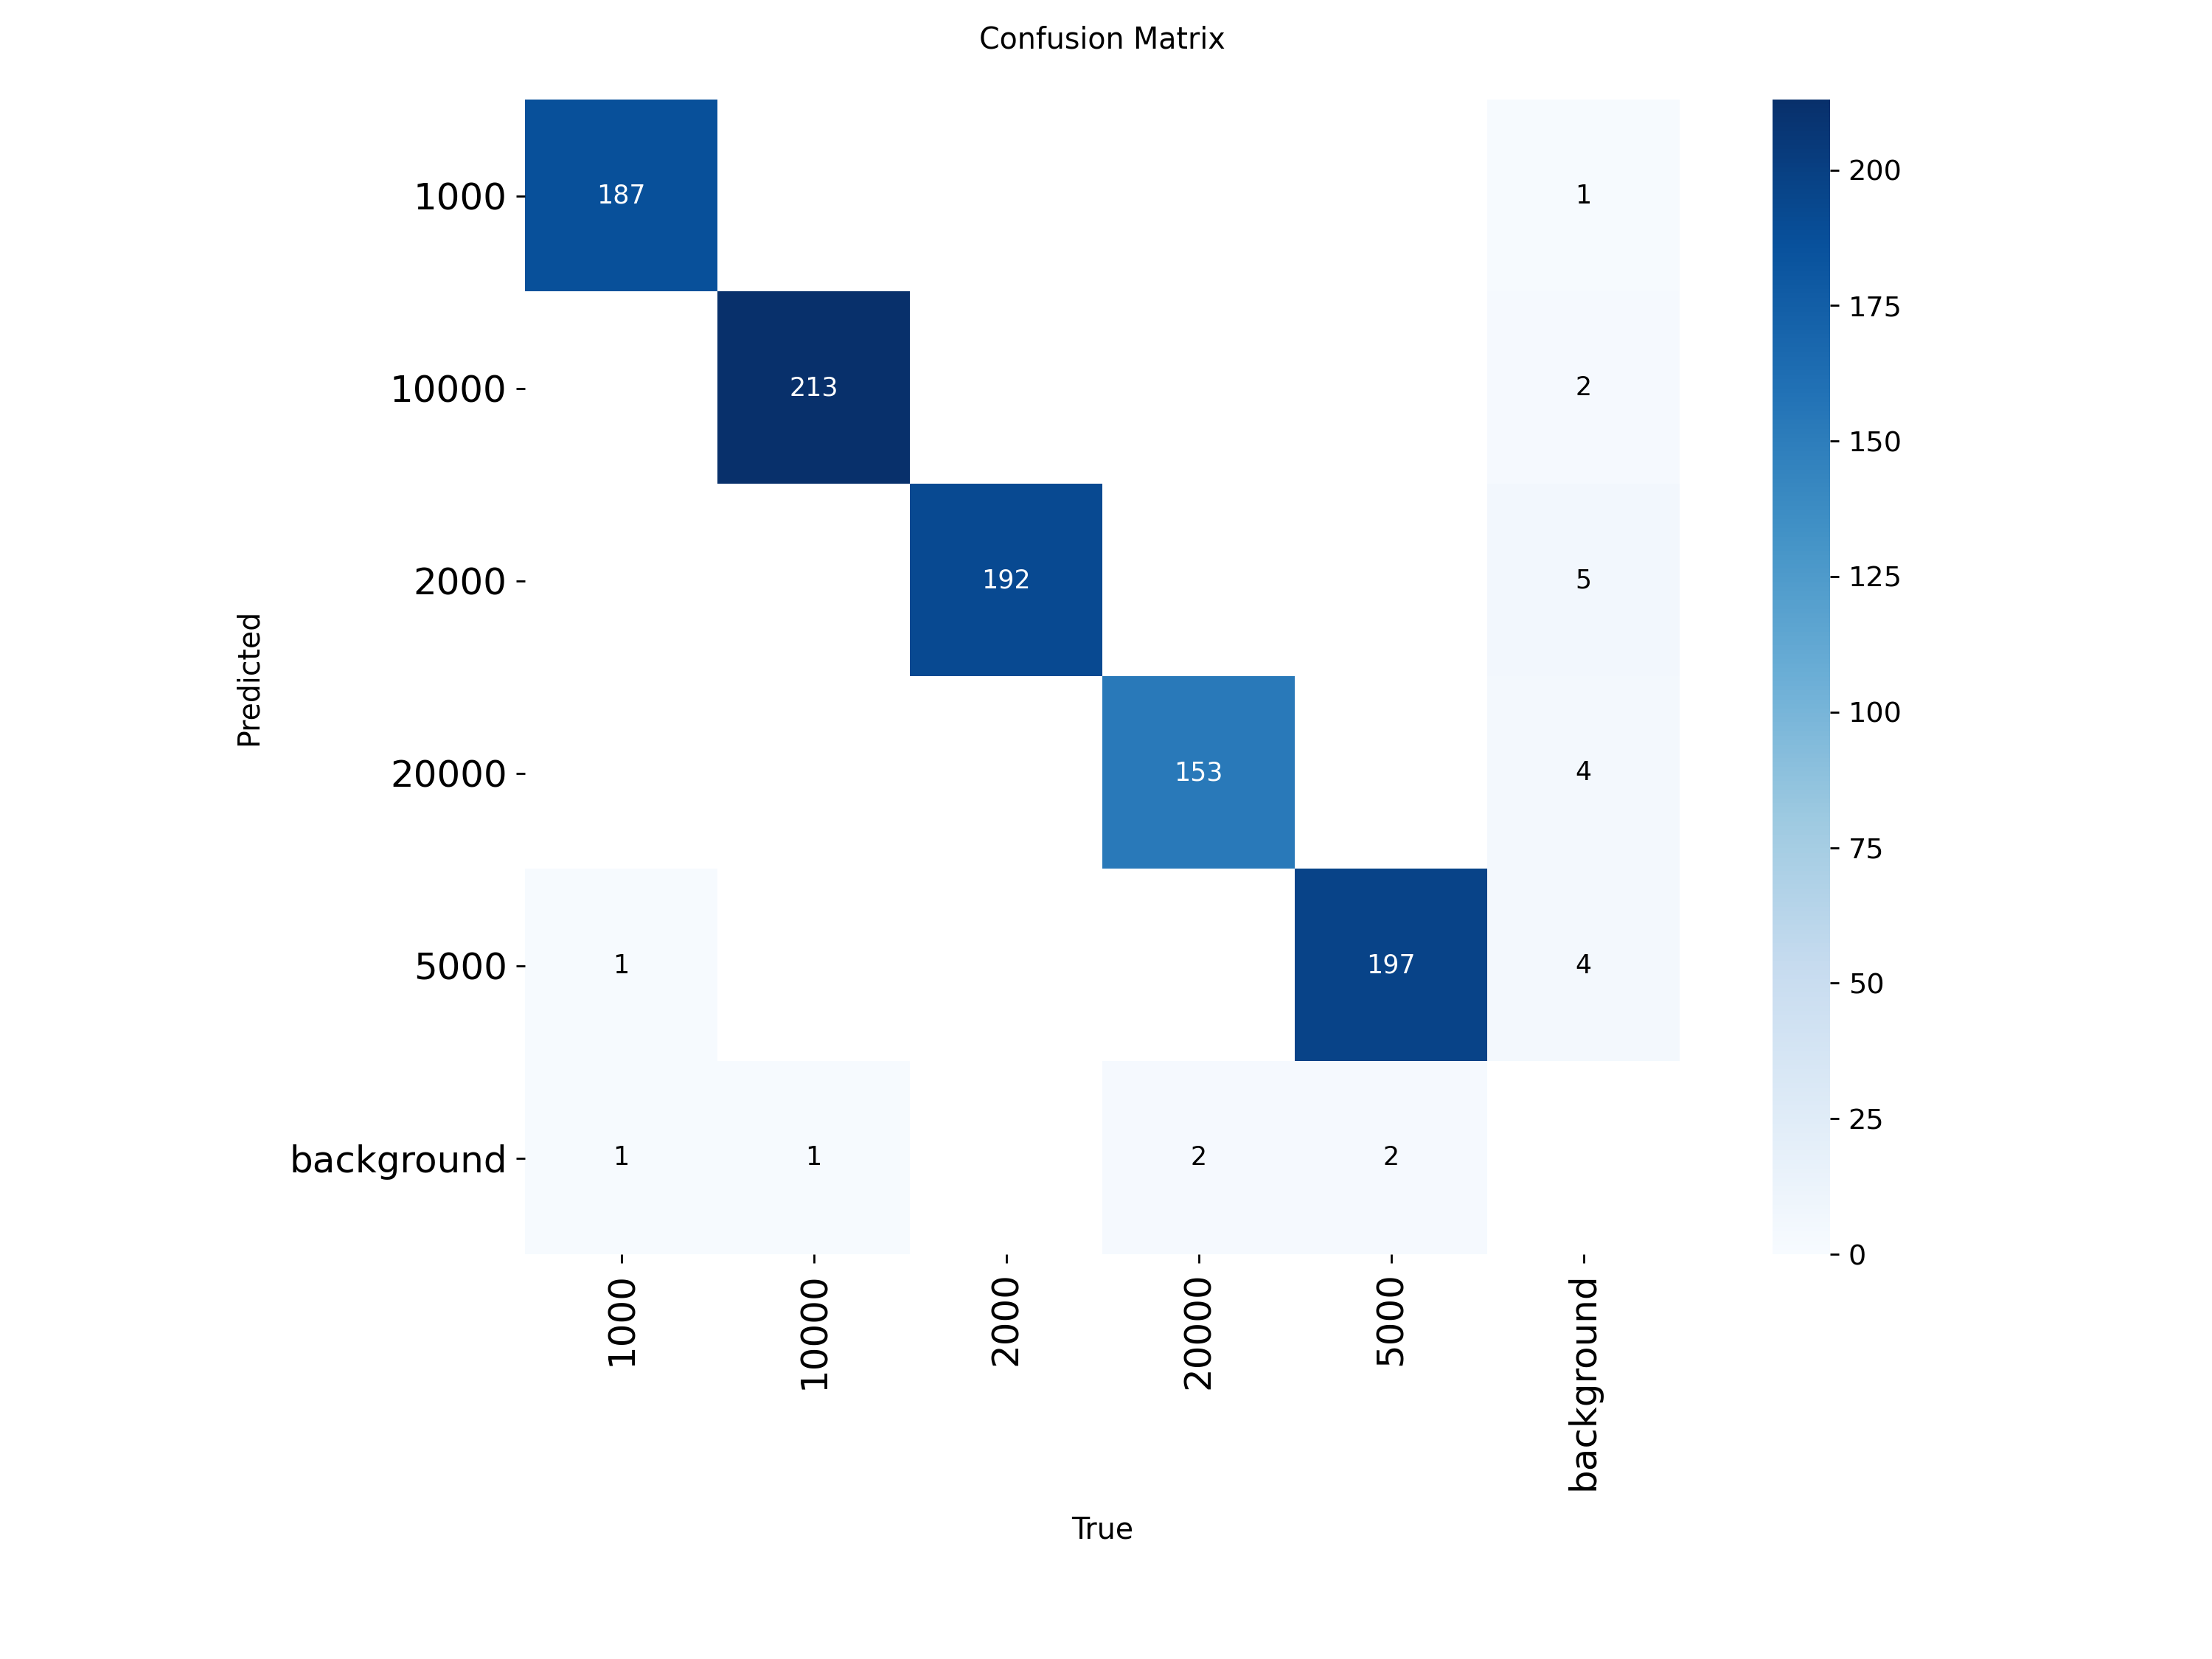
\includegraphics[width=0.8\textwidth]{../DATASETS/runs/detect/train/confusion_matrix.png}
    \caption{Matriz de confusión del modelo en el conjunto de validación.}
    \label{fig:confusion_matrix}
\end{figure}

\end{document}